We assembled block-group level data from the 2008-2012 American Community Survey (ACS), conducted by the U.S. Census Bureau, on race and ethnicity for counties corresponding to 28 large US cities. At this early stage, the counties used were chosen to correspond to the most densely populated urban cores; in future developments we could standardize to conduct analyses for Metropolitan Statistical Areas. We then aggregated the detailed racial and ethnic groups into five meta-categories: `Asian', `Black', `Hispanic', `Other', and `White'. For each city, we computed the entropy $H(Y)$ and the mutual information $I(X,Y)$. To compute the estimated aggregate Fisher information $J(X,Y)$, we tiled the map with a hexagonal grid of cell radius 1km. We then computed the estimated mutual information within each grid cell, and averaged the results weighted by population population. A technical specification of this approach is provided in Appendix 1, and a complete summary of cities and their associated information measures is provided in Appendix 3. 
		
	\begin{figure}
		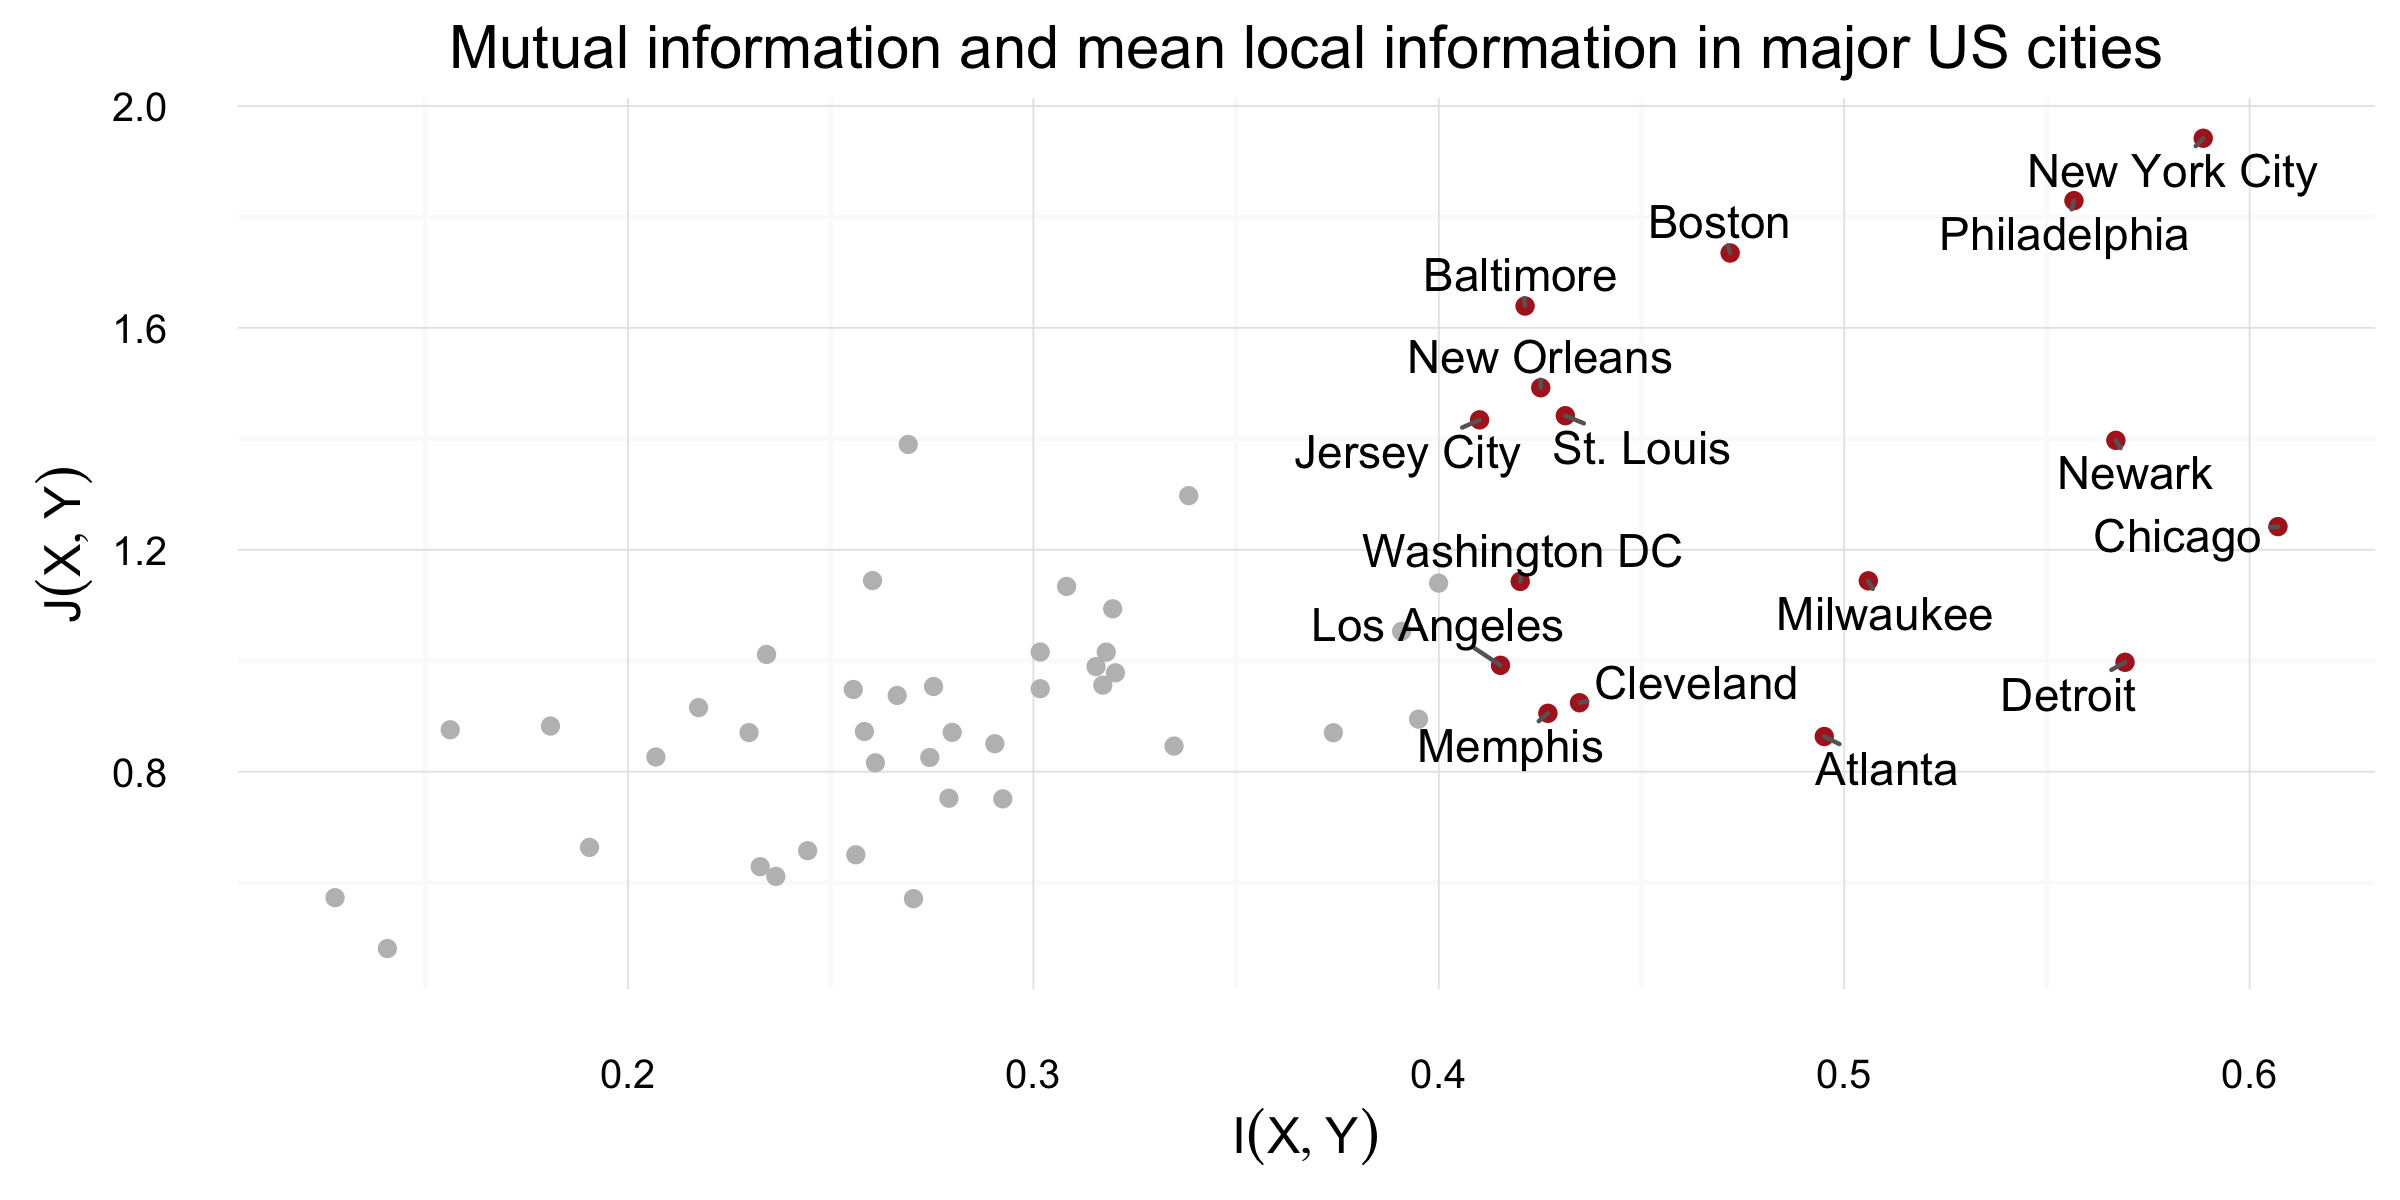
\includegraphics[width=1\textwidth]{figs/mutual_fisher.png}
		\caption{Relationship of global mutual information $I(X,Y)$ and mean local information $J(X,Y)$.} 
		\label{fig:info_cross}
	\end{figure}	
Figure \ref{fig:info_cross} shows the relationship of the global spatial variability $I(X,Y)$ and mean local variability $J(X,Y)$. An overall positive trend is evident, reflecting the fact that global spatial variability is a prerequisite for local variability: if the city is uniform (like Figure \ref{fig:toy}(a)), then no local differences either exist.  On the other hand, there are substantial variations in $J(X,Y)$ even in cities with comparable global variability $I(X,Y)$. For example, the cities of Detroit and Philadelphia provide a striking contrast. While they have comparable global variability $I(X,Y)$, Philadelphia's $J(X,Y)$ is substantially higher. This reflects the fact that Detroit is composed of large, highly-segregated, monoracial neighborhoods, whereas Philadelphia has a much more fine-grained, intricate neighborhood structure. These patterns illustrate how combinations of the information measures $H(Y)$, $I(X,Y)$, and $J(X,Y)$ can be used to construct taxonomies diversity for American cities. 

Intriguingly, the mean local variability $J(X,Y)$ appears obey a scaling relation with respect to urban density. In Figure \ref{fig:density}, we plot $J(X,Y)$ against the population density $\rho$ of our studied cities. A clear trend is evident, with $J(X,Y)$ growing linearly with the logarithm of density. We interpret this trend as reflecting a compression of social space in dense urban areas: the same structure of racial variability fits into much less geographical area in New York than in Phoenix. One aspect of diversity in large, dense cities is that one need walk much less distance in order to reach a neighborhood with substantially different racial trends than one's own. 
 
	\begin{figure}
		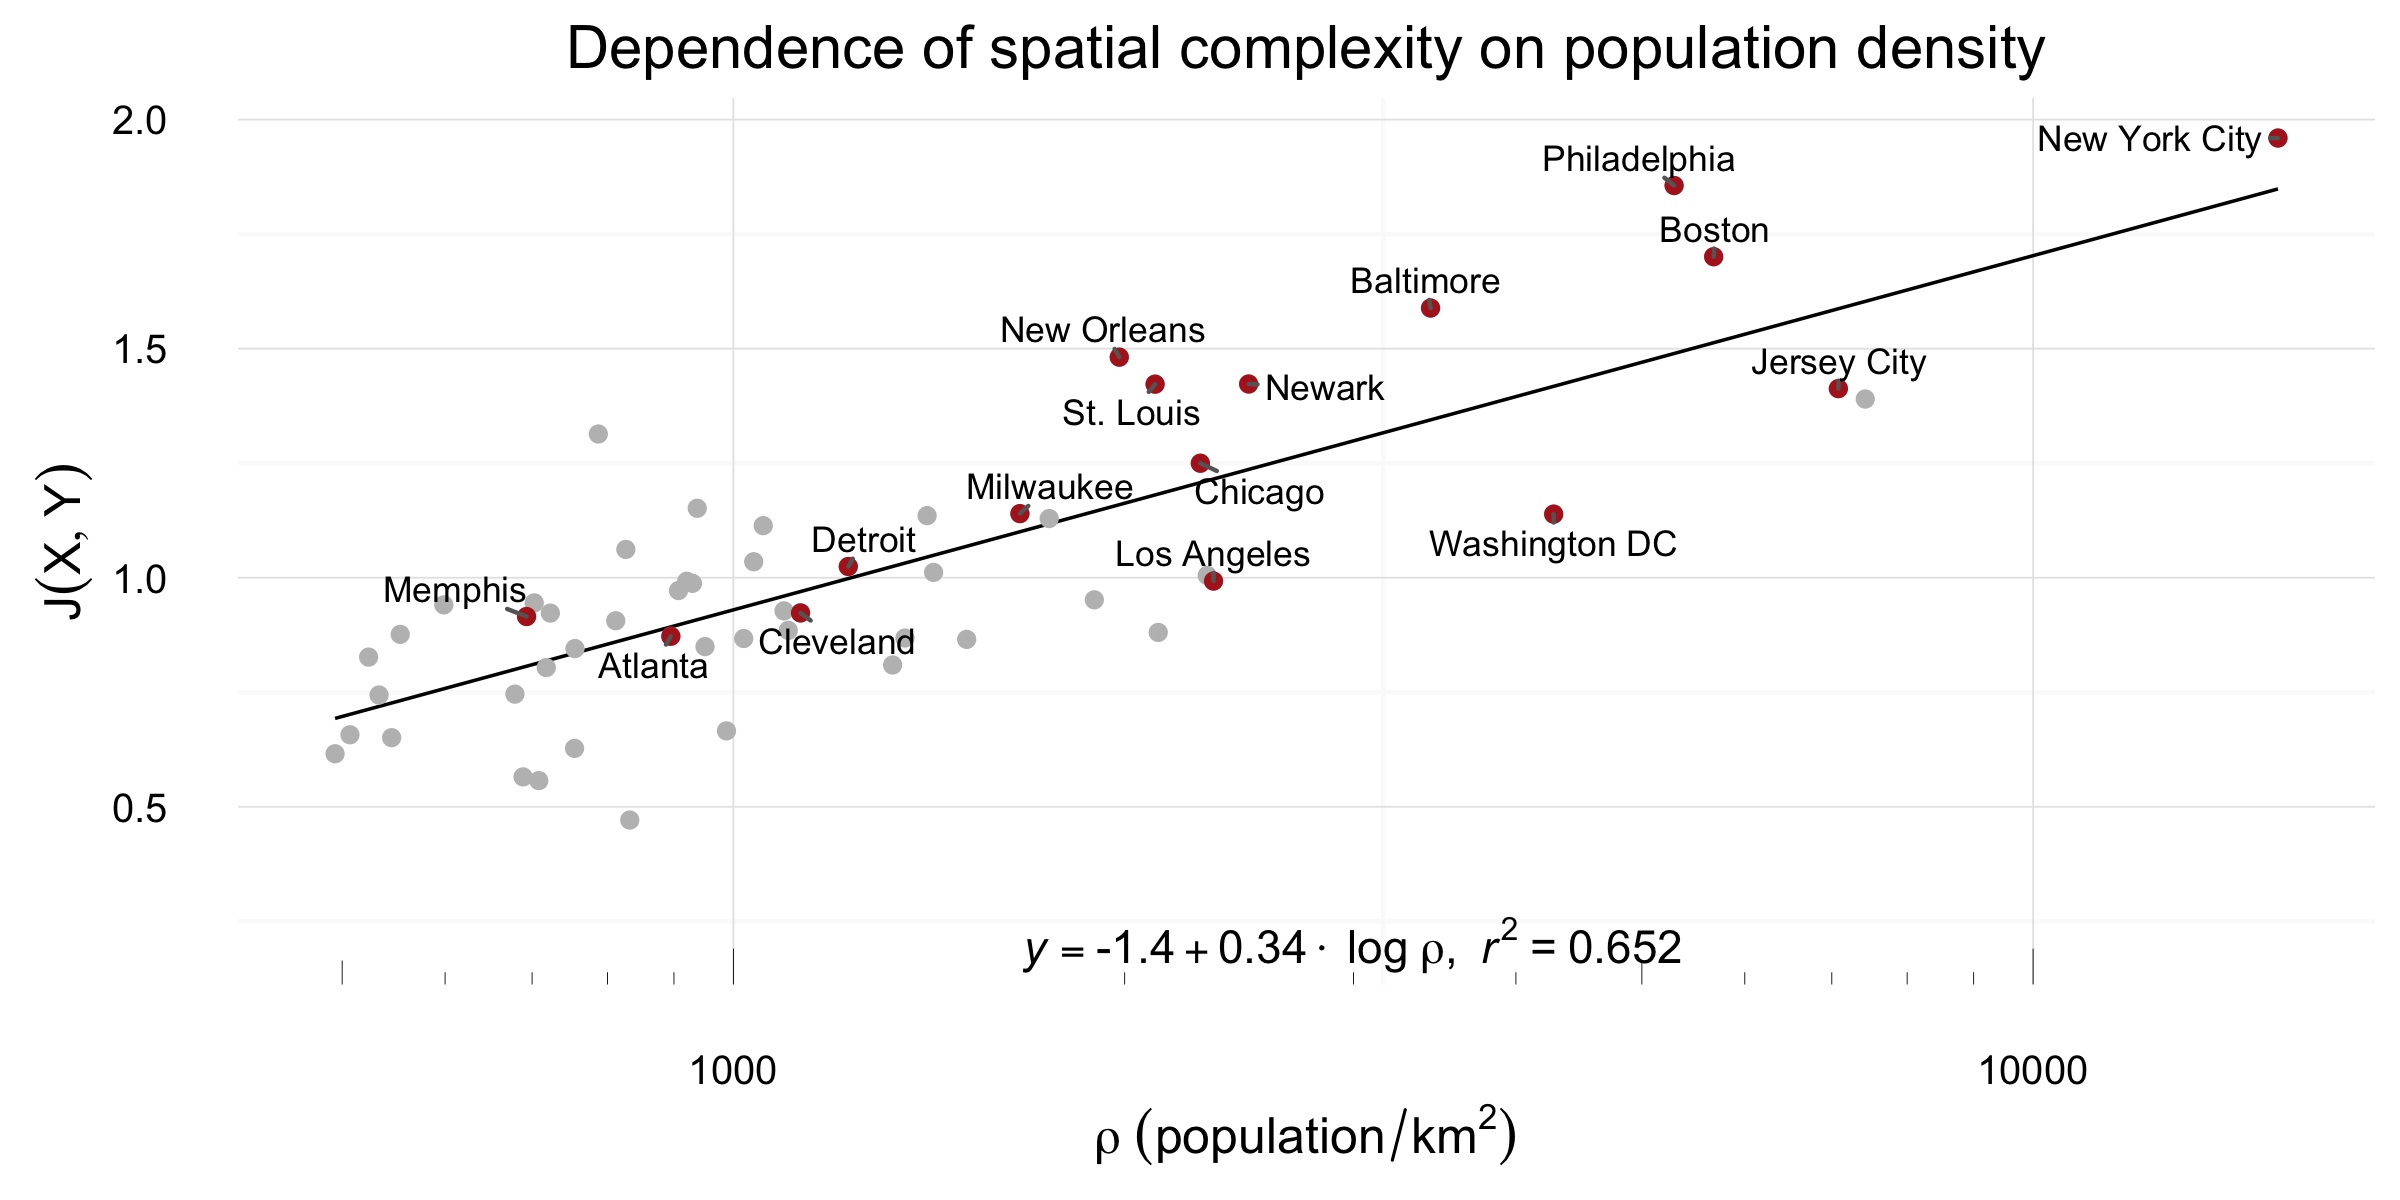
\includegraphics[width=1\textwidth]{figs/density_fisher.png}
		\caption{The mean local information $J(X,Y)$ scales with the logarithm of population density.}
		\label{fig:density}
	\end{figure}	
